% TeX root=../main.tex

\section{Sistema de escrita}

Os hieróglifos anatólicos são um sistema de escrita autóctone da Anatólia
utilizado, até onde se sabe, apenas para escrever textos em luvita.
O sistema utiliza tanto \emph{logogramas}, i.e.\ caracteres que denotam uma
unidade semântica, quanto \emph{fonogramas}, i.e.\ caracteres que denotam sons da
língua.
Há duas variedades principais dos hieróglifos, os de baixo relevo, produzidos
com incisões no material de suportes, e os de alto relevo, produzidos
desbastando a pedra em volta dos caracteres.\footnote{Neste documento, 
	caracteres dos hieróglifos anatólicos serão tipografados utilizando a fonte 
	{\tiny\texttt{Noto Sans Anatolian Hieroglyphs}}, que os representa no estilo de 
baixo relevo.}
As inscrições do período imperial utilizam sinais levemente diferentes dos
sinais das inscrições do período neo-hitita e seus escribas tendem a preferir 
o uso de logogramas em detrimento dos fonogramas.\footnote{%
	Para detalhes do sistema de escrita, vide
	\citet[pp.\ 6ff.\ e pp.\ 23ff.]{CHLI11} e \citet[pp. 354ff.]{CHLI3}.
}

	
Parte dos hieróglifos pode ter interpretação tanto de logograma quanto de
fonograma e, em alguns casos, a interpretação fonográfica surgiu por
\emph{rebus}, isto é, o logograma passou a ser utilizado para indicar parte do
som da palavra originalmente denotada por ele, como em~\Next.
Alguns sinais não estabilizaram uma leitura fonográfica quando da escrita das
inscrições que nos chegaram e ainda, por vezes, são lidos como \emph{rebus},
como em~\NNext.

\ex.\a. L.66 DARE 𔑈 = \emph{pi{(ya)}-} `dar' $\rightarrow$ /pi/
\b. L.509 (=L.329) CURRERE 𔘰 \slash{} 𔕰 = \emph{hwi{(ya)}-} `correr' $\rightarrow$
/hwi/

\ex. L.13 PRAE 𔐎 = \emph{pari} \slash{} \emph{paran} `em frente' $\rightarrow$
/pa.ri/\footnote{Como no nome próprio Parita, escrito 𔐎𔐞 PRAE-tá- =
\emph{Parita-} em QALʿAT EL MUDIQ, § 1.}

\paragraph{Transliteração e transcrição}
Por conveniência, costuma-se transliterar o texto hieroglífico no alfabeto latino
e então produzir a transcrição do que se supõe ser a forma ``corrida'' do texto.

\noindent A convenção de transliteração para o alfabeto latino consiste em:
\noprelistbreak%
\begin{compactenum}
	\item Se o sinal não tem interpretação estabelecida ou a interpretação no
		contexto é incerta, incluir o número do logograma conforme em
		\citet{LarocheHH}, seja com um asterisco ou um \emph{L.} antecedendo o
		número
	\item Se o sinal tem valor logográfico ou \emph{rebus},
		escrever o valor semântico convencional em latim,
		seguindo~\citet{LarocheHH} e letras maiúsculas.\footnote{Por vezes,
		sinais que denotam topônimos não são latinizados e são grafados em itálico.}
	\item Se um ou mais logogramas estão em função de \emph{determinativo}
		(\emph{vide sub}), eles são colocados entre parênteses.
	\item Se o sinal tem valor fonográfico, utilizar letras minúsculas.
	\item Sinais que pertencem à mesma palavra são separados por hifens.
\end{compactenum}
A transcrição seguem as seguintes convenções:
\begin{compactenum}
	\item sinais sem interpretação estabelecida ou logogramas cuja forma linguística
	subjacente é desconhecida, permanecem transliterados;
	\item sinais logográficos com interpretação conhecida são convertidos pela
	palavra que representam;
	\item sinais interpretados como \emph{rebus} são convertidos pro valor
	fonológico;
	\item os hifens são excluídos e os sinais com valor fonológico são unidos.
\end{compactenum}
Como a transcrição depende da interpretação das formas linguísticas subjacentes,
a conversão não é de um para um e depende do nossas suposições sobre a língua.
Com frequência, diferentes autores produzem diferentes transcrições para uma mesma
sequência de sinais e, quando em dúvida entre duas formas possíveis, incluem
parênteses nos pontos incertos.

\subsection{Fonogramas}

Os fonogramas dos hieróglifos anatólicos representam unidades de sílabas, sendo
também chamados de silabogramas.
Em sua maioria, eles representam sequências de V (Vogal) e CV (Consoante Vogal),
com alguns poucos representando a sequência CVCV, mas apenas quando a segunda 
sequência de \emph{consoante-vogal} representa a sílaba \emph{ra\slash{}ri}.\@
O silabário ``regular'' para o período das citadas-estado neo-hititas está 
representado em~\autoref{tab:silabariobasico} e~\autoref{tab:silabariobasicob} e
os sinais para séries CVCV estão em~\autoref{tab:CVCV}.

\paragraph{Fonogramas múltiplos}
	Sons que podem ser representadas por mais de um sinal recebem na transliteração
sinais adicionais. Utilizando por exemplo o som /a/, a forma mais comum será
transliterada <a>, a segunda mais comum pelo acento agudo <á> (=a$_2$), a terceira
pelo acento grave <à> (=a$_3$) e as demais por números subscritos, como <a$_5$>.
Formas que podem ter diversas vogais são grafadas com as opções de vogal
separadas por uma barra, < \slash{} >.

\clearpage
{
	\begin{figure}[ht]
	\makebox[\textwidth][l]{
	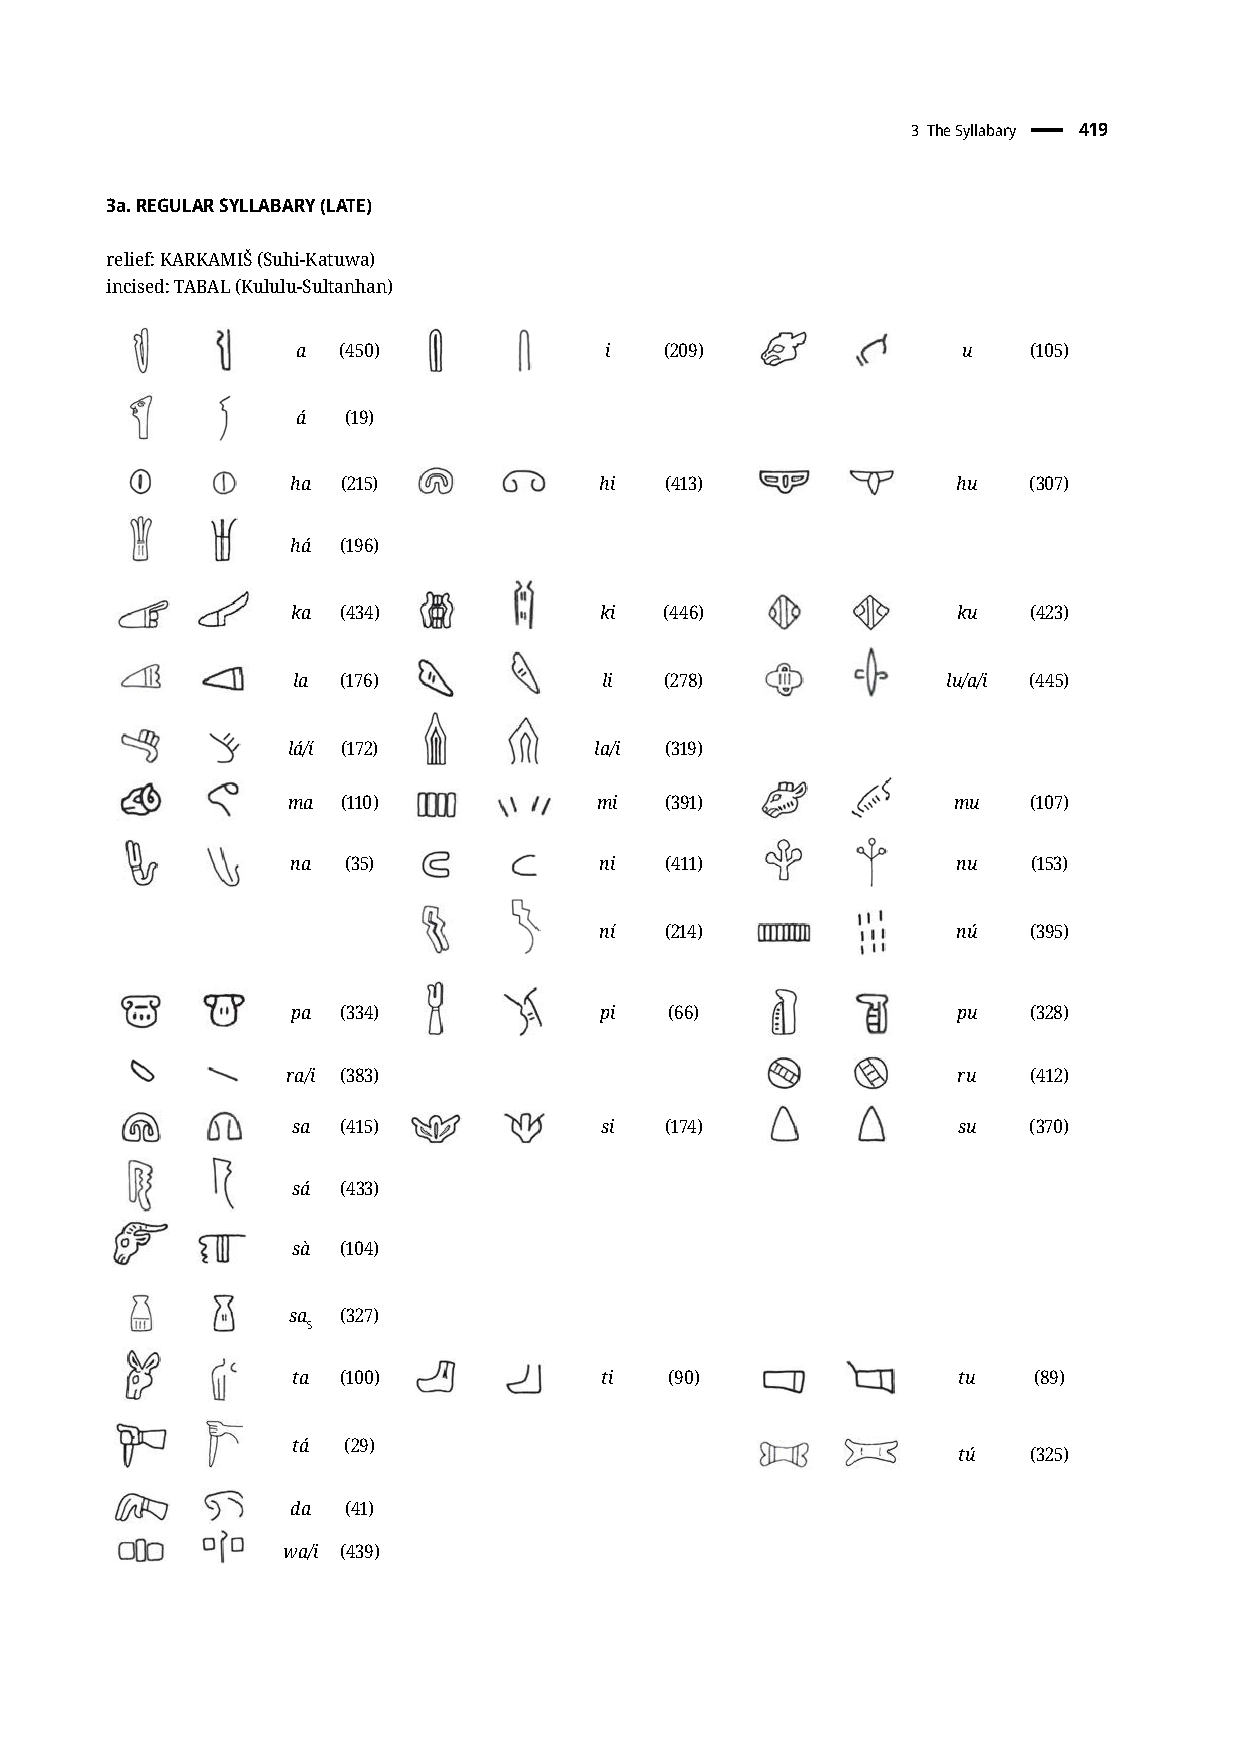
\includegraphics[width=1.2\textwidth,trim={14mm 30mm 28mm 55mm},clip]{../../Mídia/silaba.pdf}
	}
	\caption{Silabário regular~\cite[419]{CHLI3} -- Parte 1}\label{tab:silabariobasico}
\end{figure}
}
\clearpage

\clearpage
{
	\begin{figure}[ht]
		\makebox[\textwidth][r]{
	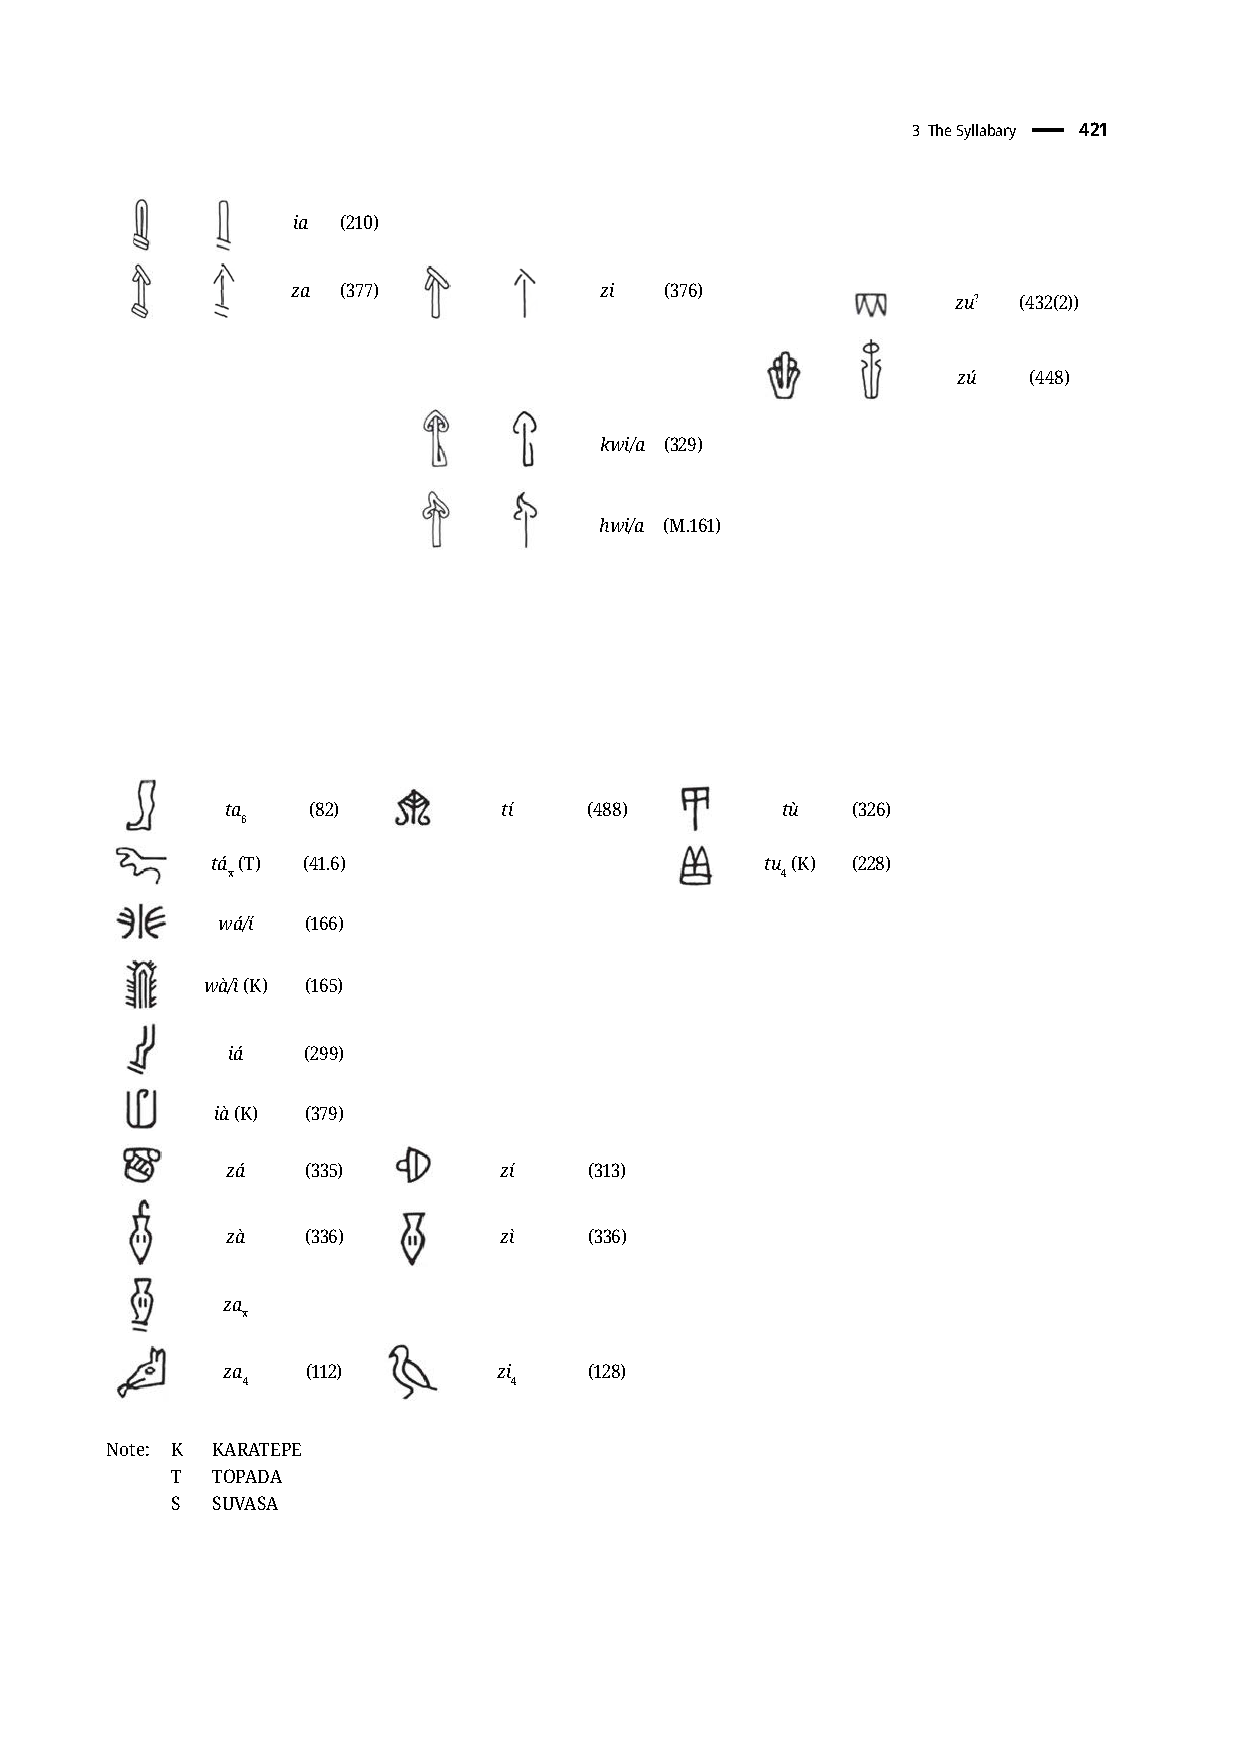
\includegraphics[width=1.2\textwidth,trim={22mm 200mm 27mm 30mm},clip]{../../Mídia/silabario-b.pdf}
	}
	\caption{Silabário regular~\cite[421]{CHLI3} -- Parte 2}\label{tab:silabariobasicob}
\end{figure}
	\begin{figure}[ht]
		\makebox[\textwidth][c]{
	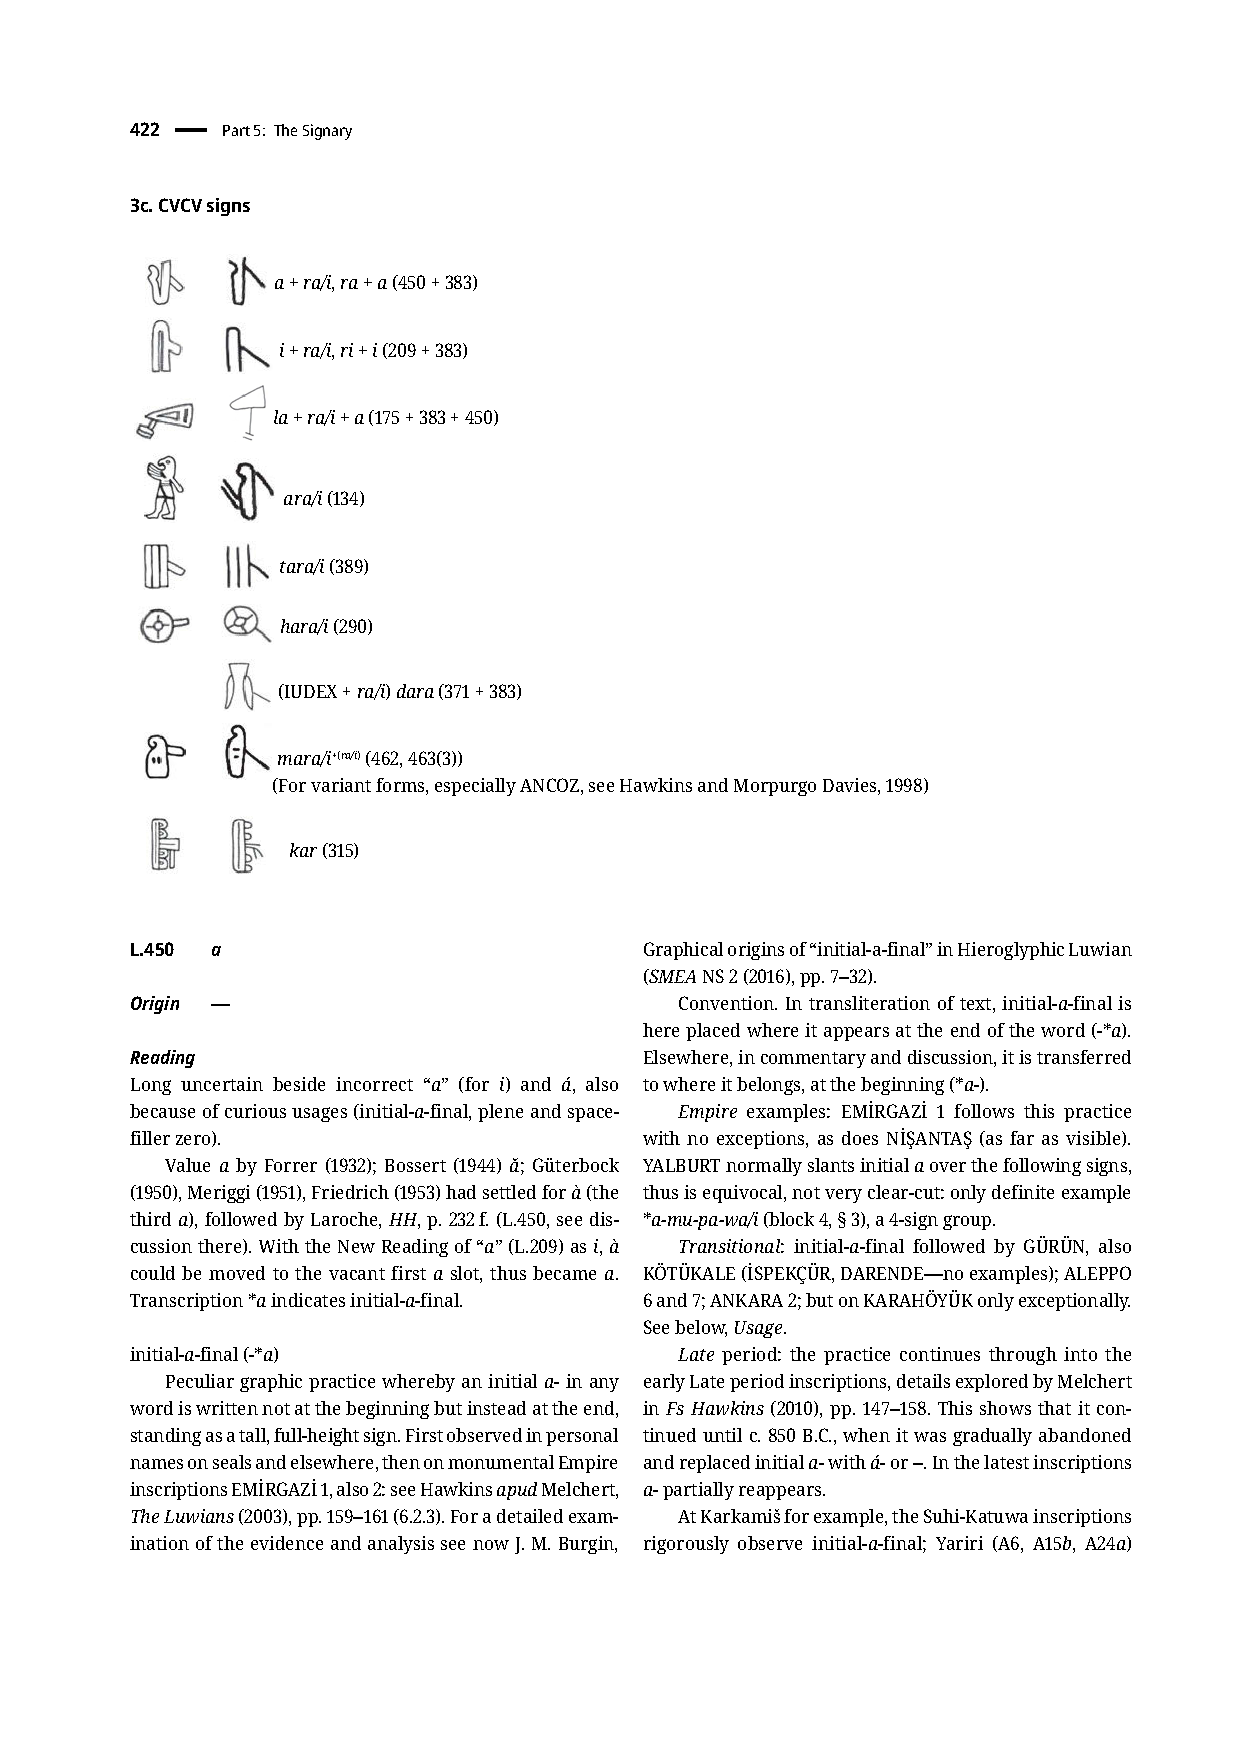
\includegraphics[width=1.1\textwidth,trim={22mm 149mm 27mm 39mm},clip]{../../Mídia/silabario-c.pdf}
	}
	\caption{Fonogramas CVCV~\cite[422]{CHLI3}}\label{tab:CVCV}
\end{figure}
}
\clearpage


\paragraph{Consoantes isoladas} 
Com esse sistema que sempre representa sequências {(C)}V, é impossível 
representar encontros consonantais e consoantes finais.
Via de regra, o costume dos escribas era de grafar uma consoante qualquer X com
o fonograma utilizado para grafar a sílaba /Xa/.
Em português, isso tornaria as palavras \emph{barco} e \emph{barraco} idênticas
na grafia, <ba-ra-co>, exigindo que o falante recuperasse pelo contexto e 
conhecimento da língua qual a forma fonológica ali
representada.\footnote{Consoantes geminadas não são representadas nos
hieróglifos anatólicos.}
Assim, para escrever \emph{hamsukalas} ``bisneto'', um escriba de MARAŞ 1 escreveu:

\exg. \ldots{} \LARGE 𔓷 \LARGE 𔒅 \LARGE 𔖢 \LARGE 𔗧 \LARGE 𔓊 \LARGE 𔗦\\
\ldots{} ha ma su ka la sá\\
\ldots{} \emph{ha\textbf{m}sukala\textbf{s}} (MARAŞ 1, §1d)

Aqui, os grafemas <ma> e <sá> devem ser interpretados como as suas respectivas
consoantes puras /m/ e /s/.

\paragraph{/n/ pré-consonantal}
Uma particularidade da escrita luvita é não grafar o /n/
pré-consonantal onde ele seria esperado pela reconstrução linguística ou
comparação com o luvita cuneiforme.\footnote{%
	Alguns interpretam nisso um sinal de que, ao menos no dialeto das inscrições
	em hieróglifos, os falantes não mais produziam a consoante /n/, mas sim
	a nasalização da vogal anterior, o que não estaria documentado nos textos
	luvitas em cuneiforme por conta ou de práticas ortográficas de escribas
	acostumados com a ortografia cuneiforme do hitita, ou de uma diferença 
	dialetal entre o dialeto da era do bronze e da era do ferro. Se for este o
	caso, o exemplo~\ref{ex:tatinzi} representaria /ta.tĩ.tsi/.}
Em português, isso tornaria as palavras \emph{manga} e \emph{maga} idênticas na
grafia, <ma-ga>.
O mesmo escriba de \Last{} para escrever a palavra para `pais' escreve:

\exg.\label{ex:tatinzi} \LARGE 𔐞 \LARGE 𔑣 \LARGE 𔖩\\
tá ti zi\\
\emph{tati\textbf{n}zi}  (MARAŞ 1, §12)

\subsection{Logogramas}

\lipsum[4]

\section{Fonologia}

\lipsum[3]

\section{Flexão nominal}

\lipsum[1]

\section{Leitura: BABYLON 3}

Trata-se de um vaso em estado fragmentário (\autoref{fig:babylon3}) escavado por
Koldewey na década de 20 onde se acredita ser a cidade de Babilônia, sítio
arqueológico de Arpada, noroeste de Alepo, contendo uma inscrição no
beiral em cursivas de baixo relevo, sentido sinistroverso, em duas linhas a
serem lidas em conjunto (para cada coluna, lê-se o caractere na primeira linha,
em seguida o da segunda linha e assim sucessivamente).
A inscrição, embora escavada na Babilônia, provavelmente teria sido
produzida em Alepo e lá dedicada ao deus do trovão Tarhunta da cidade, o que é
indicado pelo epíteto 𔓢𔑞𔕸𔗐 \textsc{tonitrus.halpa}-\textit{pa-ni}
= \textit{halpa{(wa)}ni} `halabeu', desde o período imperial,
a combinação dos logogramas L.199+L.84\slash{}85 𔓢𔑝\slash{}𔑞
\textsc{tonitrus+crus$_2$\slash{}genuflectere} 
via de regra denota a cidade de Halab.\footnote{Com L.84
	\textsc{crus}$_2$ 𔑝: ALEPPO 5; NİŞANTEPE 2, no. 57; İMAMKULU.\@
	Com L.85 \textsc{genuflectere} 𔑞:  ALEPPO 6; TELL AHMAR 5;
	KÖRKÜN;\@ BABYLON 1; BABYLON 3; \mbox{HAMA 1}.\@
 Também nomes próprios de figuras associadas a Halab são grafados com essa
 combinação, como Halparuntiya em 
 MARAŞ 1 \textsc{tonitrus.halpa}-\textit{pa-ru-ti{(-i)}-ia-}.
}
A data de produção é incerta, mas deve cair entre o século IX e VIII
\textsc{aec}.

\begin{figure}[!htb]
	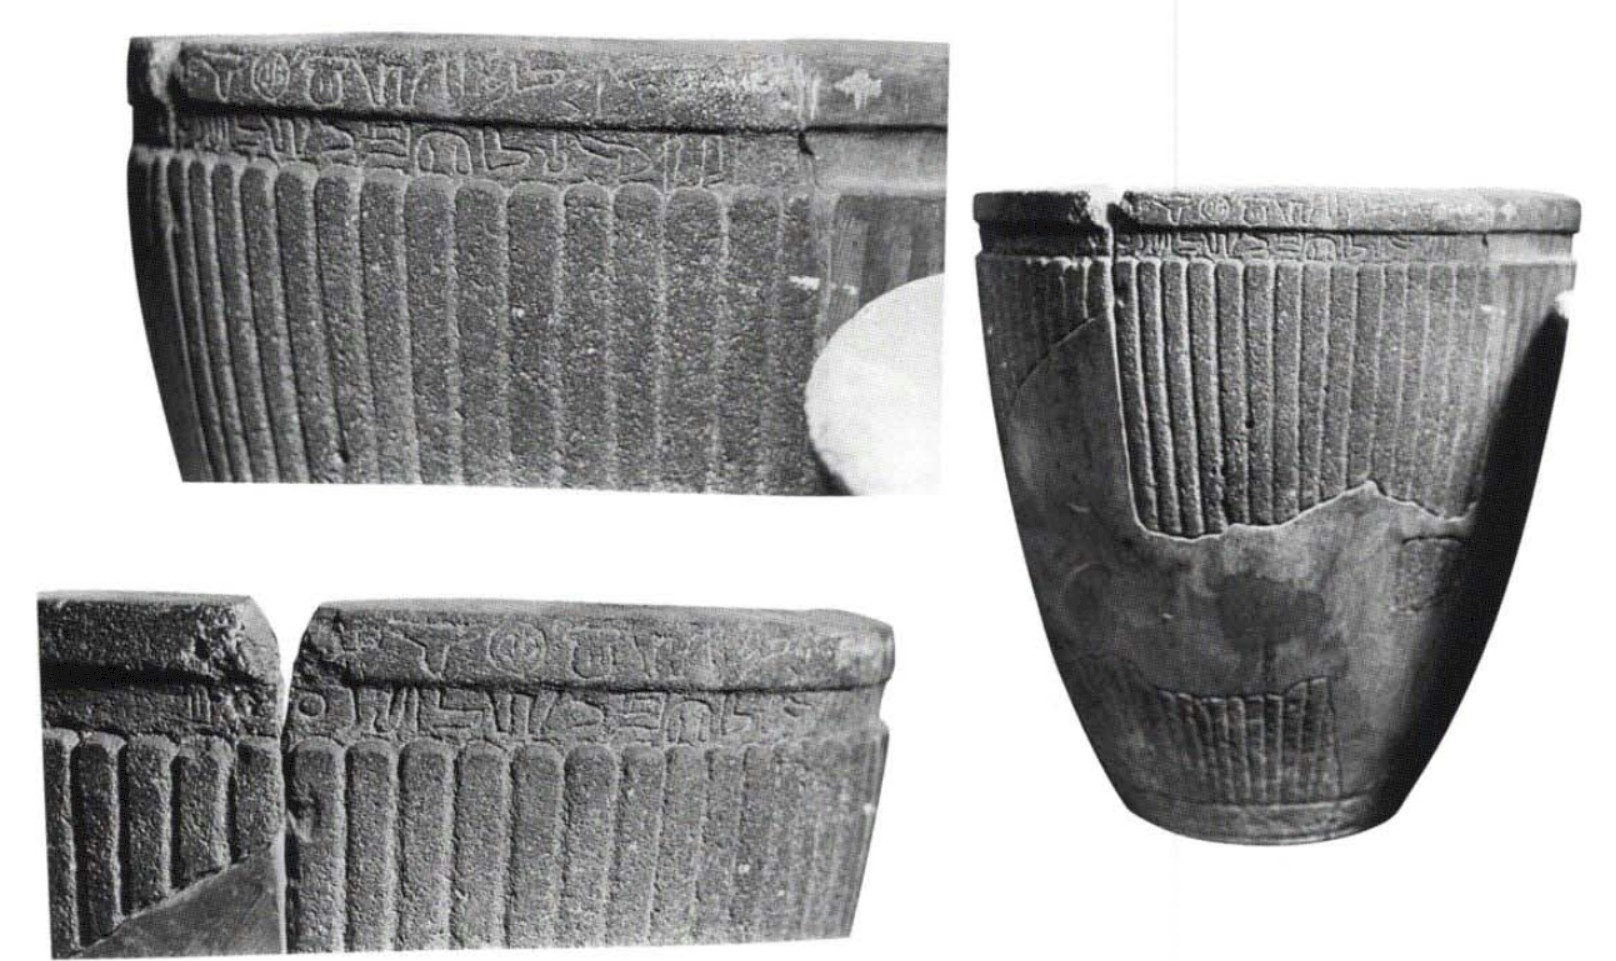
\includegraphics[width=\textwidth,trim={4mm 2mm 12mm 11mm},clip]{../../Mídia/aleppo23.jpg}
		\caption{
			Babylon 3. Diâmetro: 0.66m.; Profundidade 
			(interna): 0.67m. Imagens produzidas e traçado feito por 
			\citet[\emph{plate} 212]{CHLI13}. Atualmente no 
			\foreignlanguage{german}{Vorderasiatisches Museum}, Berlin, 
			no. VA Bab. 1507.
		}\label{fig:babylon3}
\end{figure}

	\begin{center}
		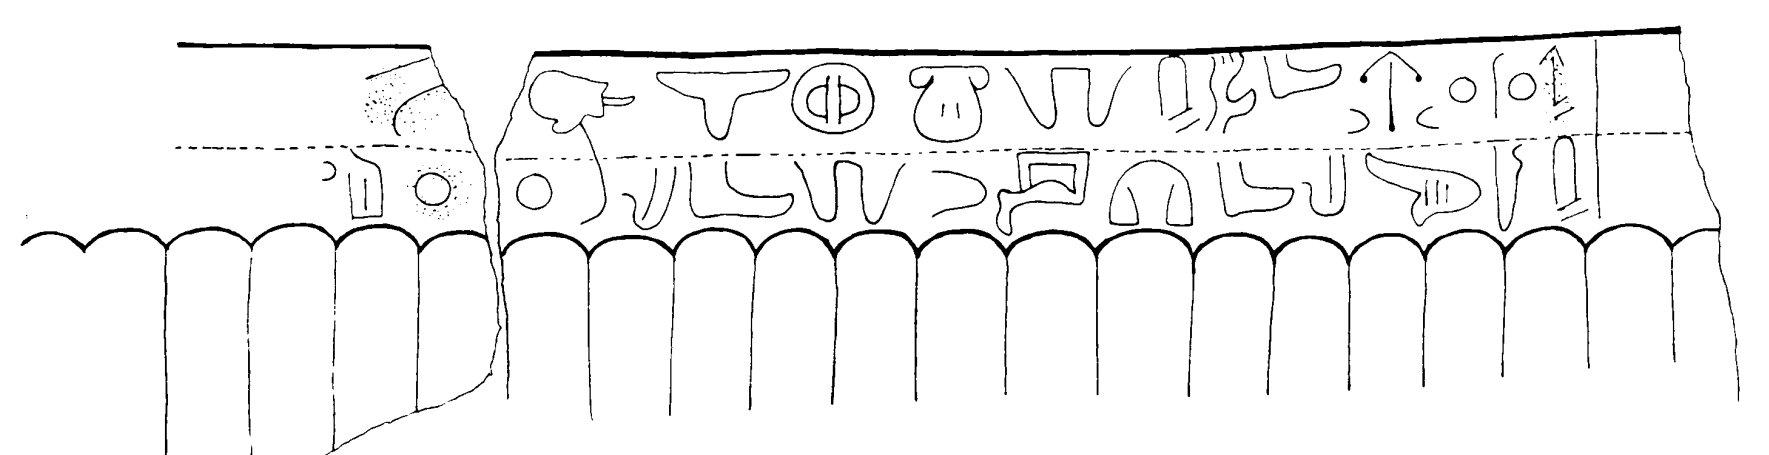
\includegraphics[width=\textwidth,trim={100mm 60mm 55mm 10mm},clip]{../../Mídia/babylon3.png}
	\end{center}
\exg.{\Large 𔖪𔓱𔗬𔗷} {\Large 𔗎𔔯𔗏𔗧𔑣𔐤} {\Large 𔑵𔑣𔓱𔗔} {\Large 𔓢𔑞𔕸𔗐} {\Large 𔖖𔓢𔕙𔑣}
{\Large 𔐎𔐤} {\Large [𔑇]𔗬𔑯}\\
za-ia-wa/i-a\hspace{10pt} ``SCALPRUM''-ka-ti-na\hspace{10pt}
CERVUS\textsubscript{2}-ti-ia-sa\hspace{10pt} TONITRUS.HALPA-pa-ni\hspace{10pt}
DEUS.TONITRUS-hu-ti\hspace{10pt} PRAE-na\hspace{10pt} [PONERE]-wa/i-ta\\
zaya=wa katin{(a)} Runtiyas halpawani Tarhu{(n)}ti paran tuwa-ta

\exg. zaya=wa katin{(a)} Runtiyas halpawani Tarhu{(n)}ti paran tuwata\\
\Det{}\Acu{} vasilha.\Neut{}\Acu{} R.\Com{}\Nom{} halabeu.\Dat{} T.\Dat{} \Prep{} colocar-3\Sg\\
Esta vaso Runtiyas dedicou ao Tarhunta halabeu.


